%======================================================================
\section{Performance evaluation}
\FloatBarrier
\subsection{Portfolio value over the backtesting period}
Figure~\ref{fig:growth} shows the value of \$1 invested in January 1998 in each portfolio, as total return net of costs. Over the 28 years the market (our S\&P 500 proxy) grows \$1 to \$12.31, the accuracy-trained timed portfolios to between \$9.46 (GJR-GARCH) and \$9.90 (GARCH-LSTM), the decision-trained GARCH-LSTM to \$9.65, and cash to \$1.78. The curves tell the main story of the project. The timed portfolios lag in strong bull markets (1998--2000, 2016--2021, 2023--2025), when they hold the market at well below full exposure after volatile spells, and they fall much less in slow crashes: in late 2002 and early 2009 buy and hold falls back below its starting value (to \$0.89 and \$0.96), while the timed portfolios stay near \$1.0 in 2002 and between \$1.4 and \$1.5 in 2009. Because the timed portfolios run at about 11\% volatility against 16\%, lower terminal wealth with a higher Sharpe ratio is the expected result: they deliver more return per unit of risk, not more return.

Figure~\ref{fig:volgrowth} adds the 12-month rolling volatility and the drawdown. The timed portfolios keep their volatility between about 4\% and 20\% while buy and hold swings between about 4\% and 31\%, and their drawdowns in 2002 and 2009 are about half as deep.

\begin{figure}[htbp]
\centering
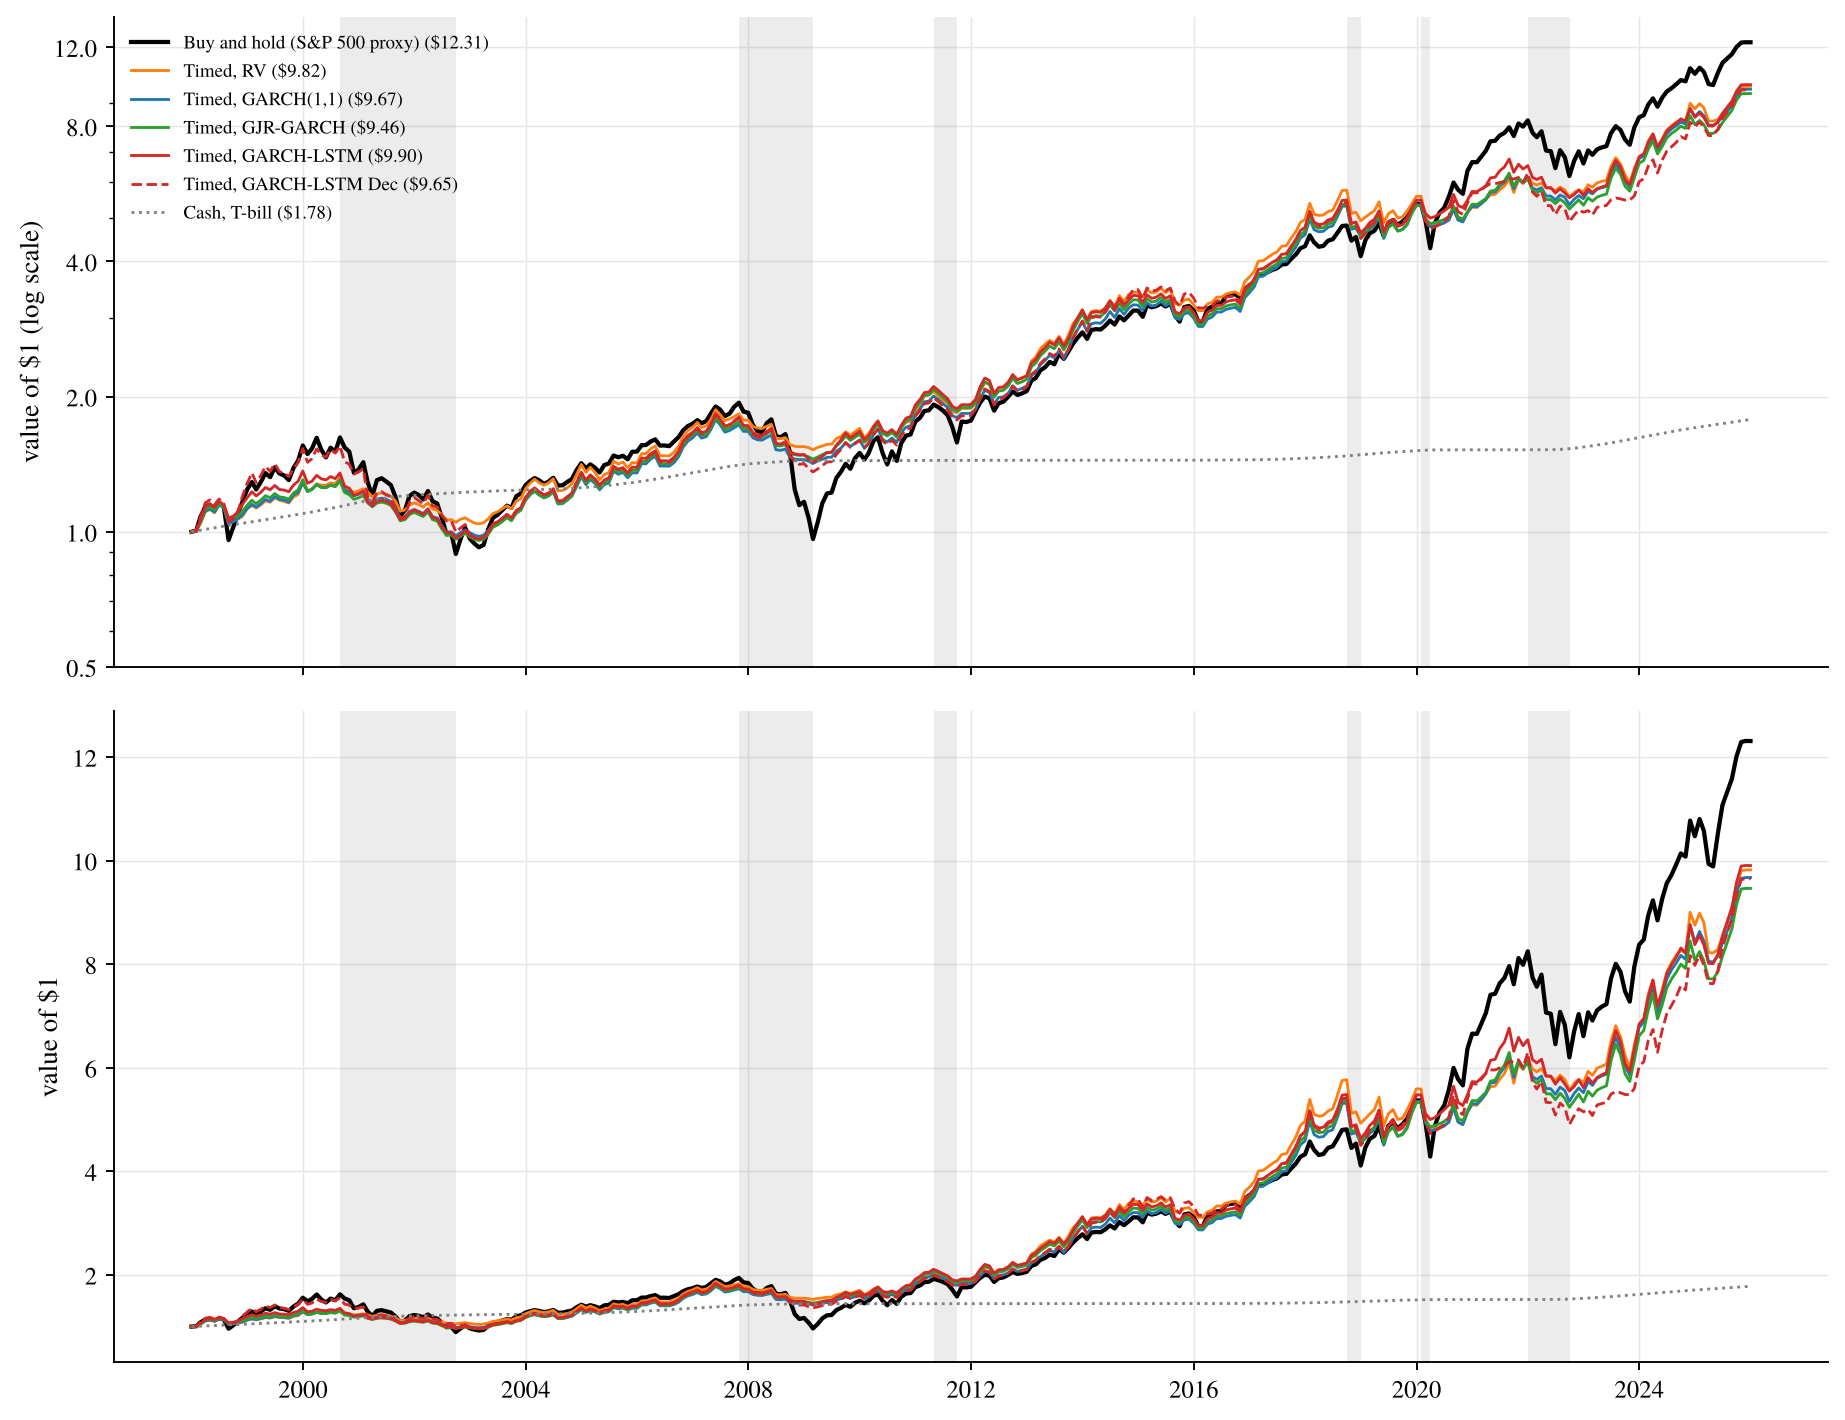
\includegraphics[width=0.93\textwidth]{figs/fig_growth.png}
\caption{Value of \$1 invested in January 1998, total return (excess return plus T-bill rate) net of 10 bp costs, log scale (top) and linear scale (bottom). Benchmark: buy and hold of the CRSP value-weighted US market (S\&P 500 proxy). ``Dec'' is the decision-trained GARCH-LSTM (Section~\ref{sec:q3}). Grey bands: the six crisis episodes.}
\label{fig:growth}
\end{figure}

\begin{figure}[htbp]
\centering
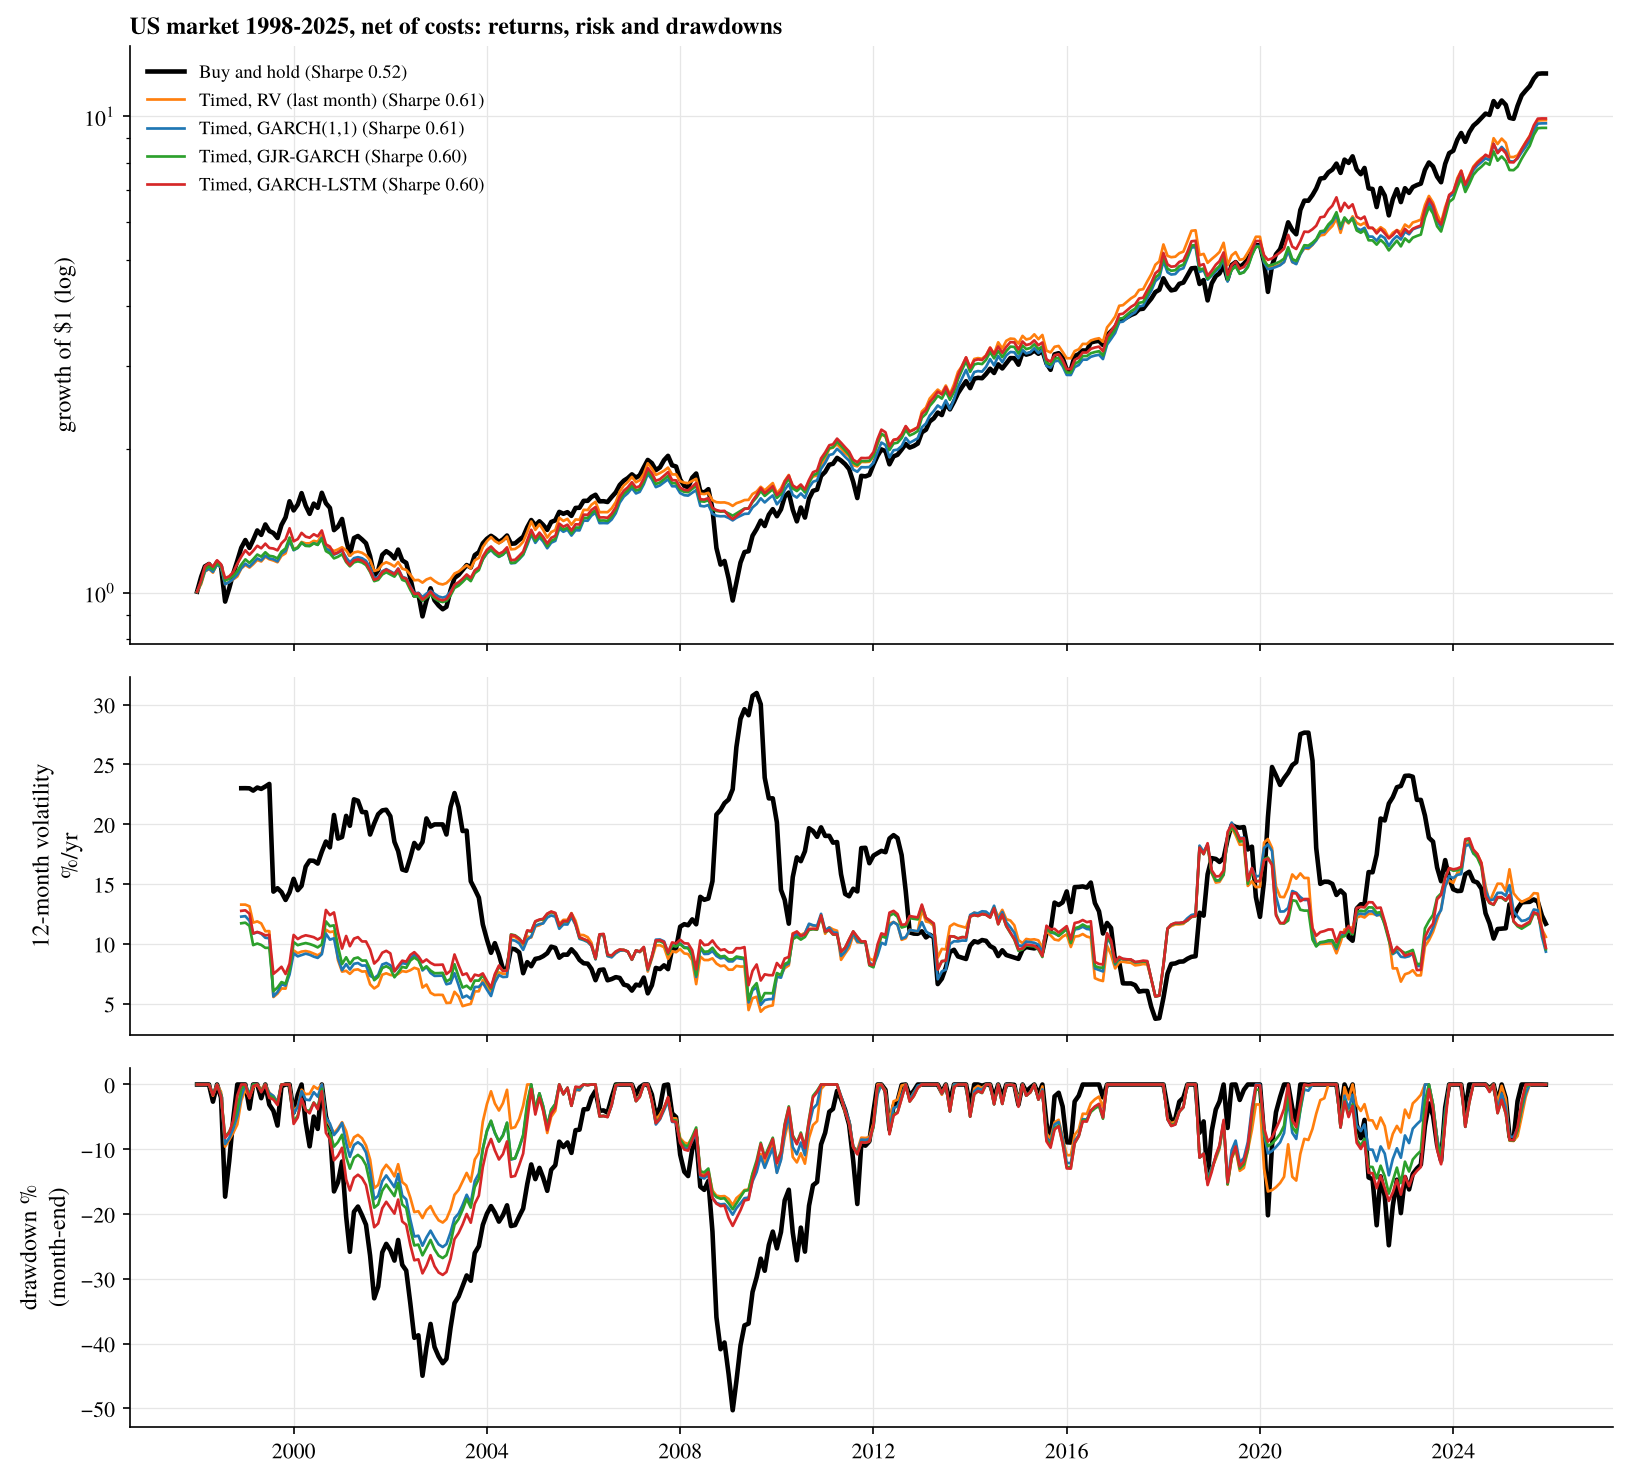
\includegraphics[width=0.85\textwidth]{figs/fig03_growth_vol_drawdown.png}
\caption{Growth of \$1 (log), 12-month rolling volatility and month-end drawdown, 1998--2025, net of costs.}
\label{fig:volgrowth}
\end{figure}

\FloatBarrier
\subsection{Performance table against the benchmark}
Table~\ref{tab:perf} reports the required metrics for the full test period.

Every accuracy-trained timed portfolio beats the S\&P 500 proxy on every risk-adjusted measure: Sharpe ratio 0.60--0.61 against 0.52, Sortino ratio 0.89--0.92 against 0.75, Calmar ratio 1.6 to 2.1 times as high, and a worst drawdown cut from $-$50\% to between $-$21\% and $-$29\%. They give up 0.8 to 1.0 points of compound annual return (1.4 to 1.6 points of mean excess return) for about 30\% less volatility, with a market beta of 0.53 to 0.58. The CAPM alpha is about 2\% a year but not significant at 5\% ($t$ between 1.6 and 1.7). Among the accuracy-trained forecasts RV, the least accurate, has the best Sharpe ratio and the smallest drawdown; GJR-GARCH and the GARCH-LSTM have the lowest Sharpe ratio (0.597). The GARCH-LSTM holds the most market on average (0.92), so it ends with the most wealth of the four but also has the deepest drawdown. Sections~\ref{sec:q2}--\ref{sec:why} explain the ordering. The decision-trained GARCH-LSTM is the weakest timed portfolio on the market (Sharpe 0.537, worst drawdown $-$37.9\%).

Figure~\ref{fig:years} shows calendar-year returns. The accuracy-trained timed portfolios beat the market in 11 to 14 of the 28 years (the decision-trained one in 12), mainly in down years (2000--2002, 2008, 2022), and lag in strong up years.

\begin{table}[htbp]
\centering\small
\caption{Portfolio performance, US market, January 1998 -- December 2025 (336 months), net of 10 bp costs.}\label{tab:perf}
\begin{adjustbox}{max width=\linewidth}\begin{tabular}{@{}lcccccc@{}}
\toprule
 & Buy and hold & \multicolumn{4}{c}{Timed, accuracy-trained forecast} & Timed\\
\cmidrule(lr){3-6}
 & (S\&P 500) & RV & GARCH & GJR & GARCH-LSTM & LSTM Dec\\
\midrule
Ann.\ return (CAGR), \% & \textbf{9.38} & 8.50 & 8.44 & 8.36 & 8.53 & 8.43\\
Ann.\ excess return (mean), \% & \textbf{8.22} & 6.73 & 6.68 & 6.61 & 6.81 & 6.89\\
Ann.\ std.\ deviation, \% & 15.93 & 11.00 & \textbf{10.99} & 11.07 & 11.40 & 12.84\\
Sharpe ratio & 0.516 & \textbf{0.612} & 0.608 & 0.597 & 0.597 & 0.537\\
Maximum drawdown, \% & $-$50.3 & \textbf{$-$21.3} & $-$25.1 & $-$26.8 & $-$29.4 & $-$37.9\\
Sortino ratio & 0.748 & \textbf{0.919} & 0.909 & 0.891 & 0.889 & 0.781\\
Calmar ratio & 0.19 & \textbf{0.40} & 0.34 & 0.31 & 0.29 & 0.22\\
Max DD at market vol, \% & $-$50.3 & \textbf{$-$32.0} & $-$36.9 & $-$39.8 & $-$41.8 & $-$46.2\\
CER ($\gamma=5$), \% p.a. & 1.87 & \textbf{3.71} & 3.66 & 3.54 & 3.56 & 2.77\\
CAPM beta & 1.00 & 0.53 & 0.55 & 0.55 & 0.58 & 0.68\\
CAPM alpha, \% ($t$) & -- & \textbf{2.37} (1.74) & 2.15 (1.67) & 2.09 (1.57) & 2.05 (1.59) & 1.33 (1.03)\\
Worst month, \% & $-$17.2 & $-$11.5 & $-$11.5 & $-$11.5 & $-$11.5 & $-$13.6\\
Value of \$1 at end, \$ & \textbf{12.31} & 9.82 & 9.67 & 9.46 & 9.90 & 9.65\\
Average exposure & 1.00 & 0.86 & 0.88 & 0.89 & 0.92 & 0.96\\
Exposure traded per year & 0.00 & 3.79 & 3.28 & 3.53 & 3.59 & 3.49\\
\bottomrule
\end{tabular}\end{adjustbox}
\par\smallskip\parbox{\textwidth}{\footnotesize Returns are total returns (CAGR) or excess returns over the T-bill (mean), annualised from monthly data; drawdowns are on month-end wealth. Alpha $t$-statistics use Newey--West standard errors (5 lags). Cash (T-bill) CAGR: 2.08\%. Best value in each row in bold. LSTM Dec: decision-trained GARCH-LSTM (Section~\ref{sec:q3}).}
\end{table}

\begin{figure}[htbp]
\centering
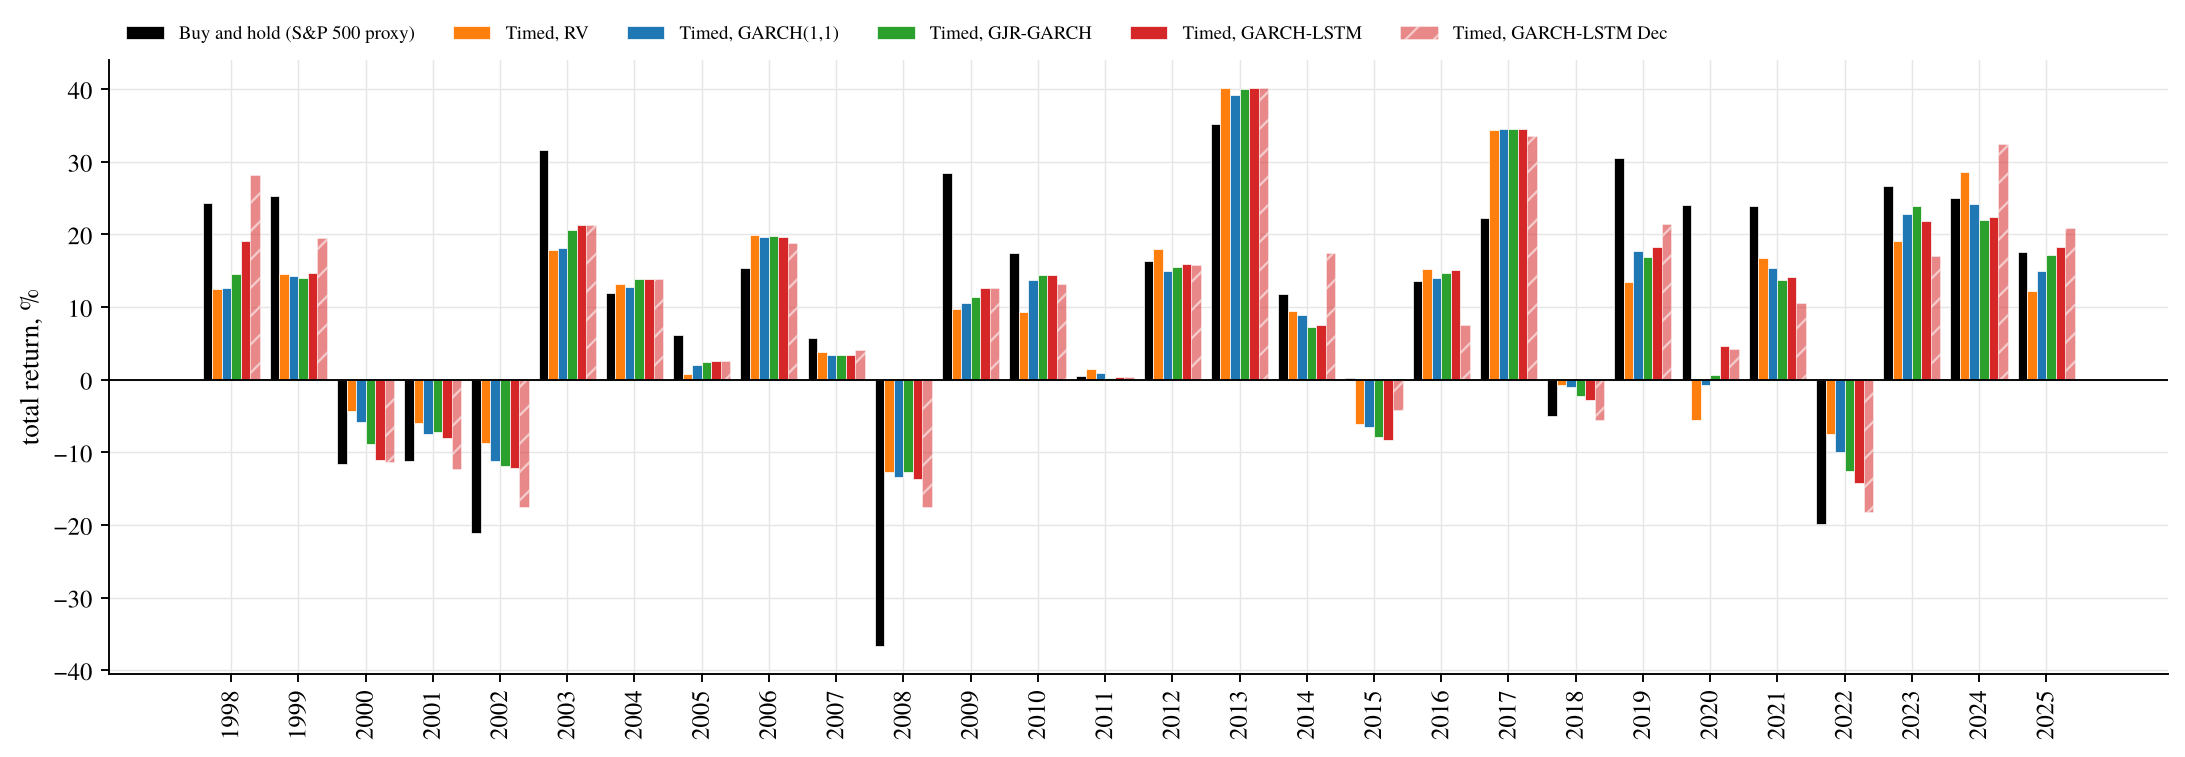
\includegraphics[width=\textwidth]{figs/fig_years.png}
\caption{Calendar-year total returns, net of costs, 1998--2025.}
\label{fig:years}
\end{figure}

\FloatBarrier
\subsection{Sub-periods}
The gain is concentrated in 1998--2015, a period with two deep bear markets, when the timed Sharpe ratio is 0.45--0.50 against 0.35 and the timed portfolios roughly match the market's compound return with about 35\% less volatility. Over 2016--2025 the accuracy-trained timed portfolios are level with or slightly behind buy and hold on the Sharpe ratio (0.78--0.83 against 0.82) and earn 2 to 3 points a year less (Table~\ref{tab:sub}). Figure~\ref{fig:rolling} shows the same pattern in the rolling 36-month Sharpe ratio: the timed portfolios are ahead in and after the 2000--2002 and 2008--2009 bear markets and behind in the long bull market of the 2010s.

\begin{table}[htbp]
\centering\small
\caption{Performance by sub-period, net of costs: CAGR (\%), annualised volatility (\%), Sharpe ratio and maximum drawdown within the period (\%).}\label{tab:sub}
\setlength{\tabcolsep}{4pt}
\begin{adjustbox}{max width=\linewidth}\begin{tabular}{@{}lcccccccccccc@{}}
\toprule
 & \multicolumn{4}{c}{1998--2015} & \multicolumn{4}{c}{2016--2025} & \multicolumn{4}{c}{2021--2025}\\
\cmidrule(lr){2-5}\cmidrule(lr){6-9}\cmidrule(lr){10-13}
 & CAGR & Vol & SR & MDD & CAGR & Vol & SR & MDD & CAGR & Vol & SR & MDD\\
\midrule
Buy and hold (S\&P 500) & 6.5 & 16.0 & 0.348 & $-$50.3 & 14.7 & 15.7 & 0.824 & $-$24.8 & 13.1 & 15.3 & 0.679 & $-$24.8\\
Timed, RV & 6.7 & 9.9 & 0.499 & $-$21.3 & 11.8 & 12.8 & 0.781 & $-$16.5 & 13.2 & 12.2 & 0.828 & $-$12.1\\
Timed, GARCH(1,1) & 6.3 & 9.9 & 0.460 & $-$25.1 & 12.5 & 12.7 & 0.828 & $-$15.3 & 12.8 & 12.1 & 0.800 & $-$14.0\\
Timed, GJR-GARCH & 6.3 & 10.1 & 0.459 & $-$26.8 & 12.1 & 12.7 & 0.803 & $-$16.8 & 12.0 & 12.3 & 0.734 & $-$16.8\\
Timed, GARCH-LSTM & 6.4 & 10.5 & 0.454 & $-$29.4 & 12.4 & 12.8 & 0.815 & $-$18.0 & 11.6 & 12.5 & 0.695 & $-$18.0\\
Timed, GARCH-LSTM Dec & 6.9 & 12.6 & 0.431 & $-$37.9 & 11.3 & 13.3 & 0.718 & $-$22.1 & 11.1 & 12.1 & 0.681 & $-$22.1\\
\bottomrule
\end{tabular}\end{adjustbox}
\end{table}

\begin{figure}[htbp]
\centering
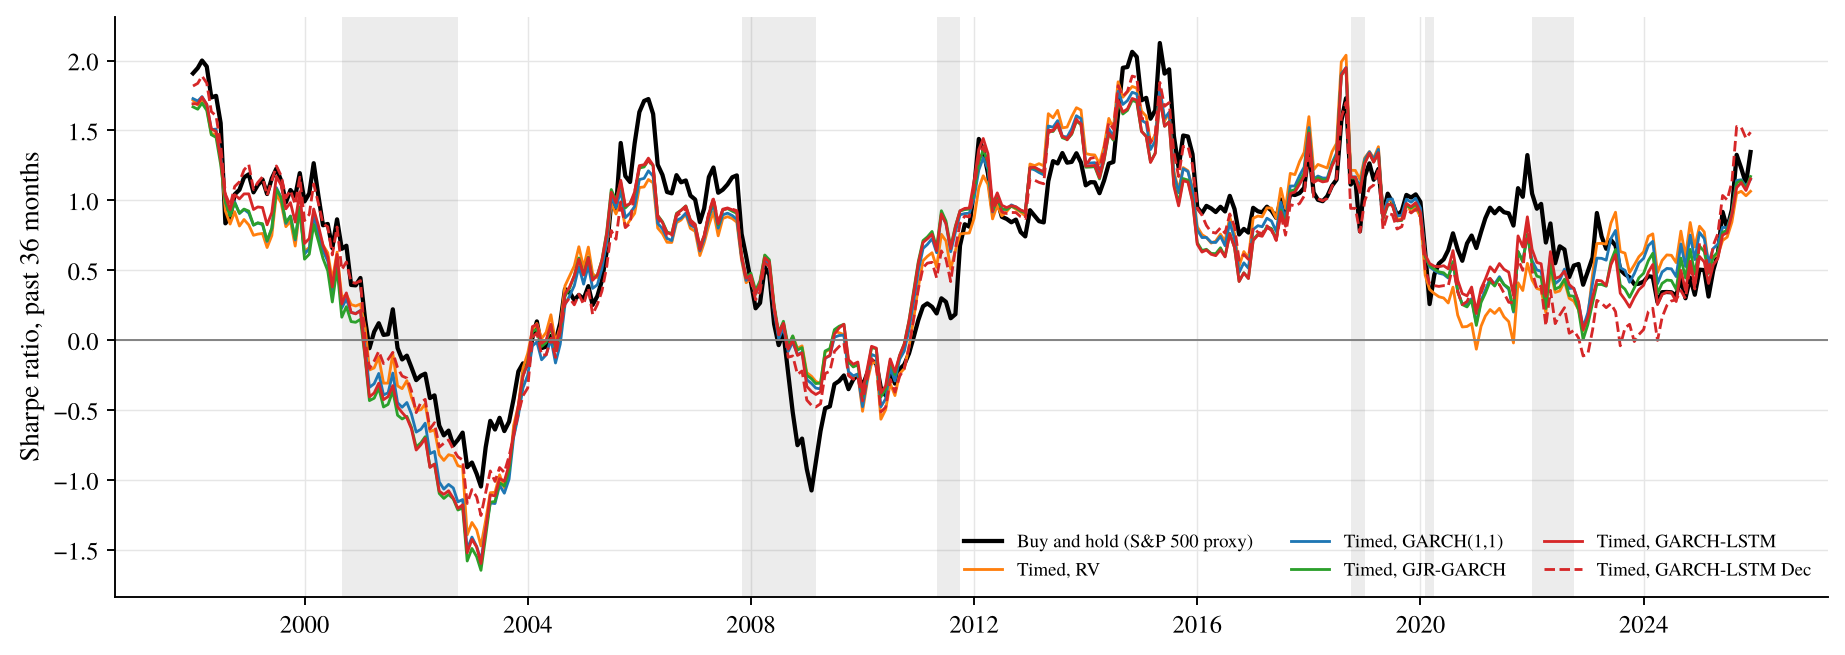
\includegraphics[width=0.9\textwidth]{figs/fig_rolling_sharpe.png}
\caption{Rolling 36-month Sharpe ratio, net of costs.}
\label{fig:rolling}
\end{figure}

\FloatBarrier
\subsection{Crisis episodes}
In five of the six episodes all four timed portfolios lost less than buy and hold, typically about half as much (Table~\ref{tab:crises}, Figure~\ref{fig:crises}). The exception is the sudden Q4 2018 sell-off ($-$14.6\% to $-$15.5\% against $-$14.5\%), which followed a calm summer with high exposure, so the forecast had no time to react. The price of protection is the rebound: in the month after each episode the exposure is only 0.02 to 0.34, so the rules miss much of the recovery (Section~\ref{sec:why}). The GARCH-LSTM and GJR-GARCH lost least in the Covid crash ($-$8.7\% and $-$8.8\%), and the GARCH-LSTM lost most of the timed rules in the dot-com and financial crises ($-$28.4\% and $-$20.3\%).

\begin{table}[htbp]
\centering\small
\caption{Total return over each crisis episode, \%, as traded, net of costs, and the exposure held in the month after the episode.}\label{tab:crises}
\setlength{\tabcolsep}{4.5pt}
\begin{adjustbox}{max width=\linewidth}\begin{tabular}{@{}lccccc|cccc@{}}
\toprule
 & \multicolumn{5}{c|}{Return over the episode, \%} & \multicolumn{4}{c}{Exposure in the month after}\\
Episode & Buy \& hold & RV & GARCH & GJR & LSTM & RV & GARCH & GJR & LSTM\\
\midrule
Dot-com (2000-09 to 2002-09) & $-$45.0 & $-$20.6 & $-$24.9 & $-$25.9 & $-$28.4 & 0.18 & 0.20 & 0.18 & 0.19\\
Financial (2007-11 to 2009-02) & $-$50.3 & $-$16.9 & $-$18.0 & $-$17.6 & $-$20.3 & 0.14 & 0.14 & 0.12 & 0.16\\
Euro (2011-05 to 2011-09) & $-$17.6 & $-$10.2 & $-$10.5 & $-$10.7 & $-$10.8 & 0.19 & 0.20 & 0.17 & 0.19\\
Q4 2018 & $-$14.5 & $-$14.6 & $-$14.6 & $-$15.1 & $-$15.5 & 0.20 & 0.22 & 0.25 & 0.27\\
Covid (2020-02 to 2020-03) & $-$20.2 & $-$13.9 & $-$10.6 & $-$8.8 & $-$8.7 & 0.02 & 0.03 & 0.04 & 0.05\\
Bear 2022 (2022-01 to 2022-09) & $-$24.8 & $-$9.9 & $-$12.6 & $-$14.2 & $-$15.2 & 0.29 & 0.34 & 0.28 & 0.17\\
\bottomrule
\end{tabular}\end{adjustbox}
\end{table}

\begin{figure}[htbp]
\centering
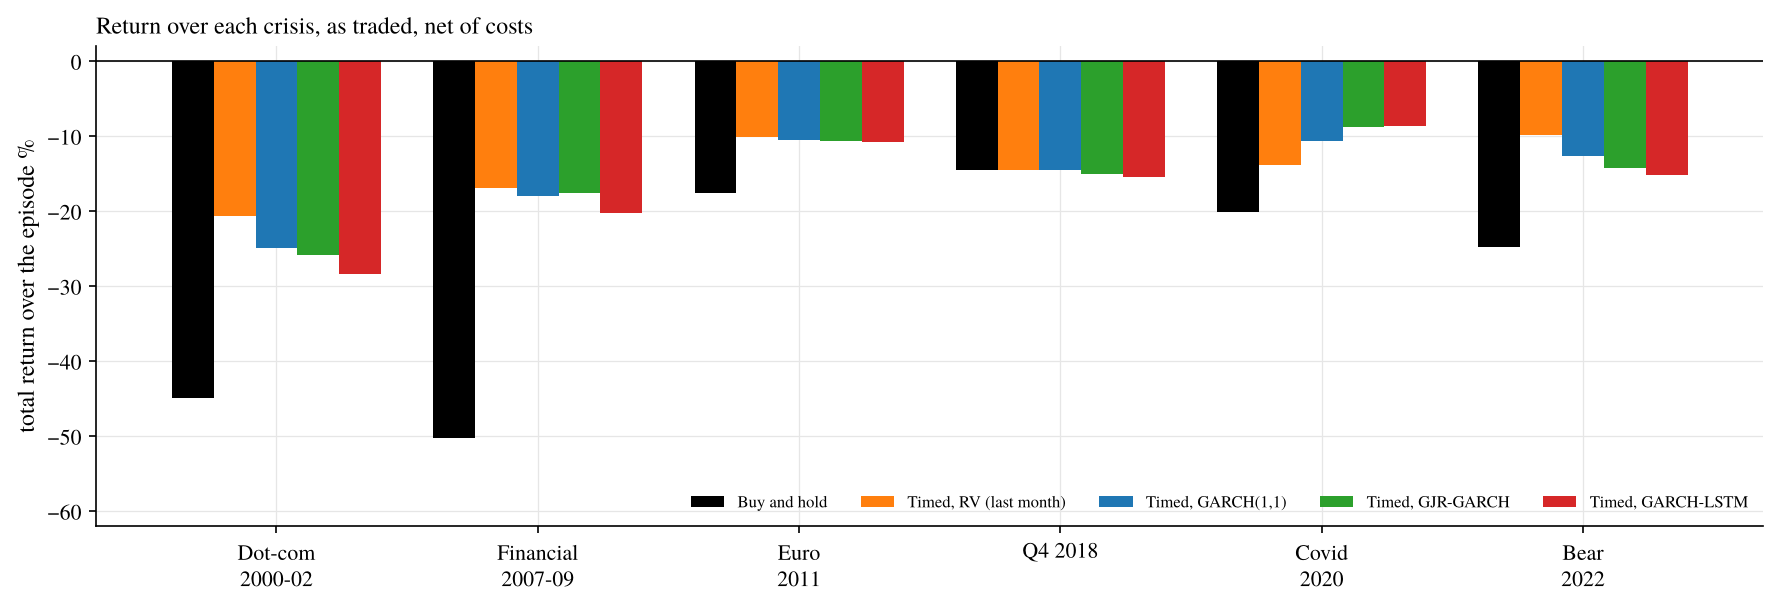
\includegraphics[width=0.85\textwidth]{figs/fig03_crises.png}
\caption{Total return over each crisis episode, as traded, net of costs.}
\label{fig:crises}
\end{figure}

\FloatBarrier
\subsection{Q1: what improves, and is it significant?}
Timing is meant to be a risk tool, so we test five measures, timed minus buy and hold (Table~\ref{tab:q1}, Figure~\ref{fig:improves}).

\begin{table}[htbp]
\centering\small
\caption{Timed minus buy and hold, 1998--2025; block-bootstrap $p$-values in brackets. Positive = better for the timed portfolio. ``Equal vol'': timed returns rescaled after the fact to buy and hold's volatility.}\label{tab:q1}
\begin{adjustbox}{max width=\linewidth}\begin{tabular}{@{}lcccc@{}}
\toprule
 & RV & GARCH(1,1) & GJR-GARCH & GARCH-LSTM\\
\midrule
Sharpe ratio & $+$0.10 (0.48) & $+$0.09 (0.44) & $+$0.08 (0.51) & $+$0.08 (0.48)\\
Sortino ratio & $+$0.17 (0.48) & $+$0.16 (0.45) & $+$0.14 (0.51) & $+$0.14 (0.49)\\
Max DD at equal vol, pts & $+$18.3 (0.10) & $+$13.4 (0.14) & $+$10.6 (0.26) & $+$8.5 (0.35)\\
Vol of vol at equal vol, pts & $+$1.2 (0.09) & \textbf{$+$1.6 (0.03)} & \textbf{$+$1.8 (0.02)} & \textbf{$+$2.1 (0.005)}\\
CER, \% p.a. & $+$1.8 (0.44) & $+$1.8 (0.41) & $+$1.7 (0.44) & $+$1.7 (0.40)\\
Sharpe: Ledoit--Wolf $p$ & 0.49 & 0.47 & 0.53 & 0.50\\
Sharpe: Romano--Wolf $p$ & 0.61 & 0.59 & 0.61 & 0.61\\
\bottomrule
\end{tabular}\end{adjustbox}
\end{table}

\begin{figure}[htbp]
\centering
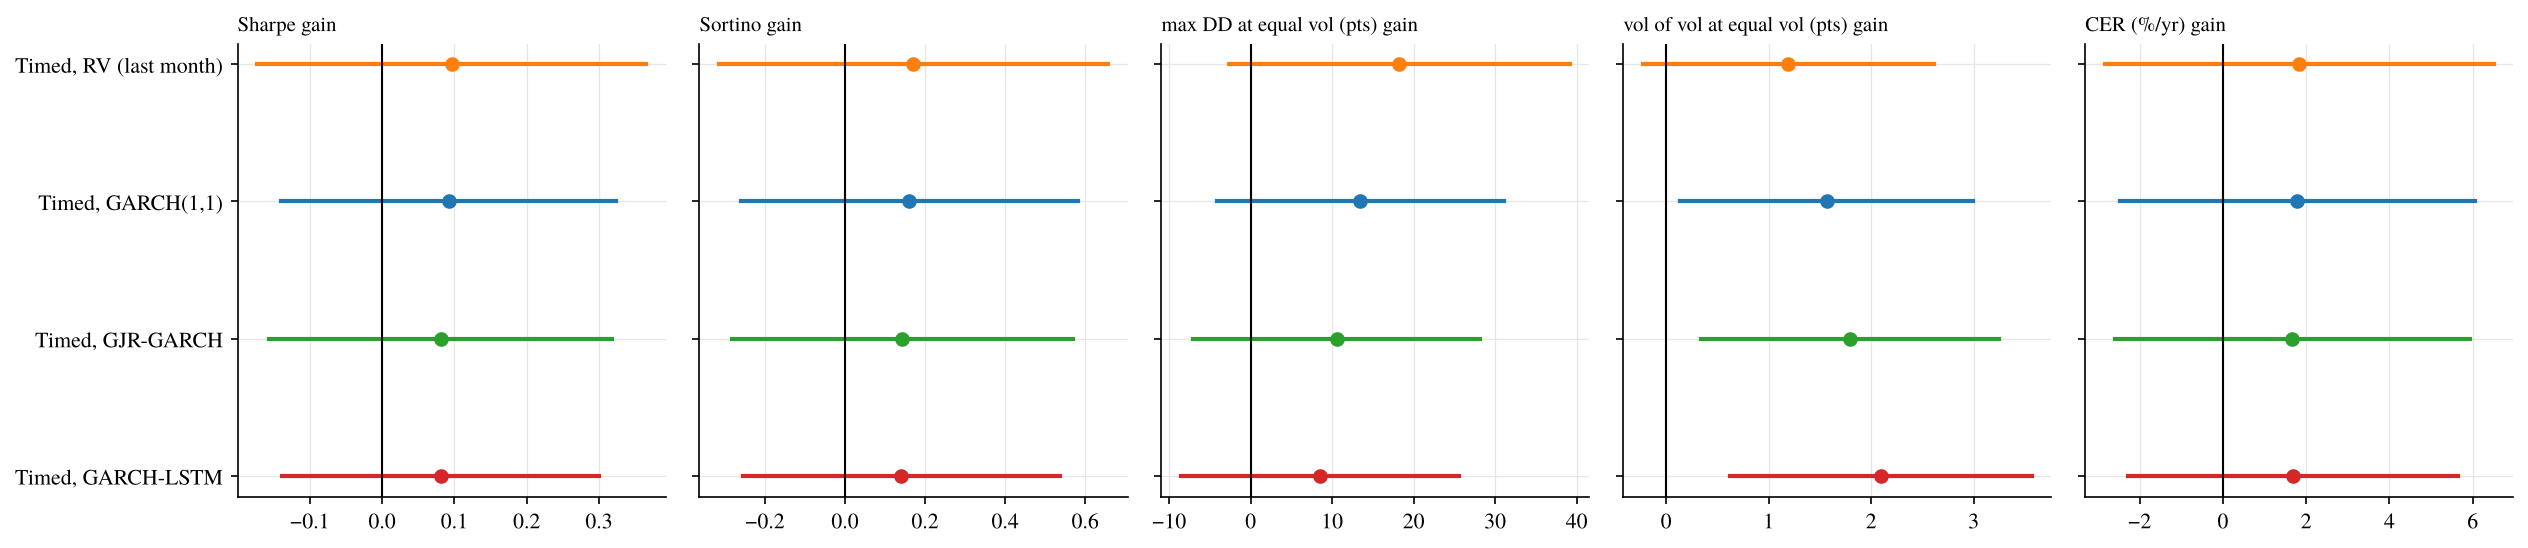
\includegraphics[width=\textwidth]{figs/fig03_what_improves.png}
\caption{What timing improves: timed minus buy and hold, 1998--2025, with 95\% block-bootstrap intervals (right of zero = better).}
\label{fig:improves}
\end{figure}

\begin{itemize}
\item \textbf{Drawdowns.} At equal volatility the timed portfolios' worst drawdown is 8 to 18 points smaller ($-$32\% to $-$42\% against $-$50\%), and as traded it roughly halves. The intervals include zero ($p$ 0.10 to 0.35): with one 28-year history and a handful of crashes, a drawdown difference is hard to prove.
\item \textbf{Steadier risk.} Rescaled to the same volatility, the GARCH(1,1), GJR-GARCH and GARCH-LSTM portfolios have a vol of vol 1.6 to 2.1 points lower than buy and hold (3.7\% to 4.2\% against 5.8\%), with intervals that exclude zero ($p$ 0.005 to 0.033, before adjusting for four rules). This is the only statistically significant improvement, and exactly what an inverse-variance rule is designed to deliver.
\item \textbf{Sharpe ratio.} $+$0.08 to $+$0.10, not significant with either test, before or after the Romano--Wolf adjustment, in any period: $+$0.11 to $+$0.15 in 1998--2015 and $-$0.04 to $+$0.00 in 2016--2025 (Figure~\ref{fig:byperiod}).
\end{itemize}
\textit{Answer to Q1: yes on risk, no on return.} Timing makes the ride smoother; it does not make the investor reliably richer per unit of risk.

\begin{figure}[htbp]
\centering
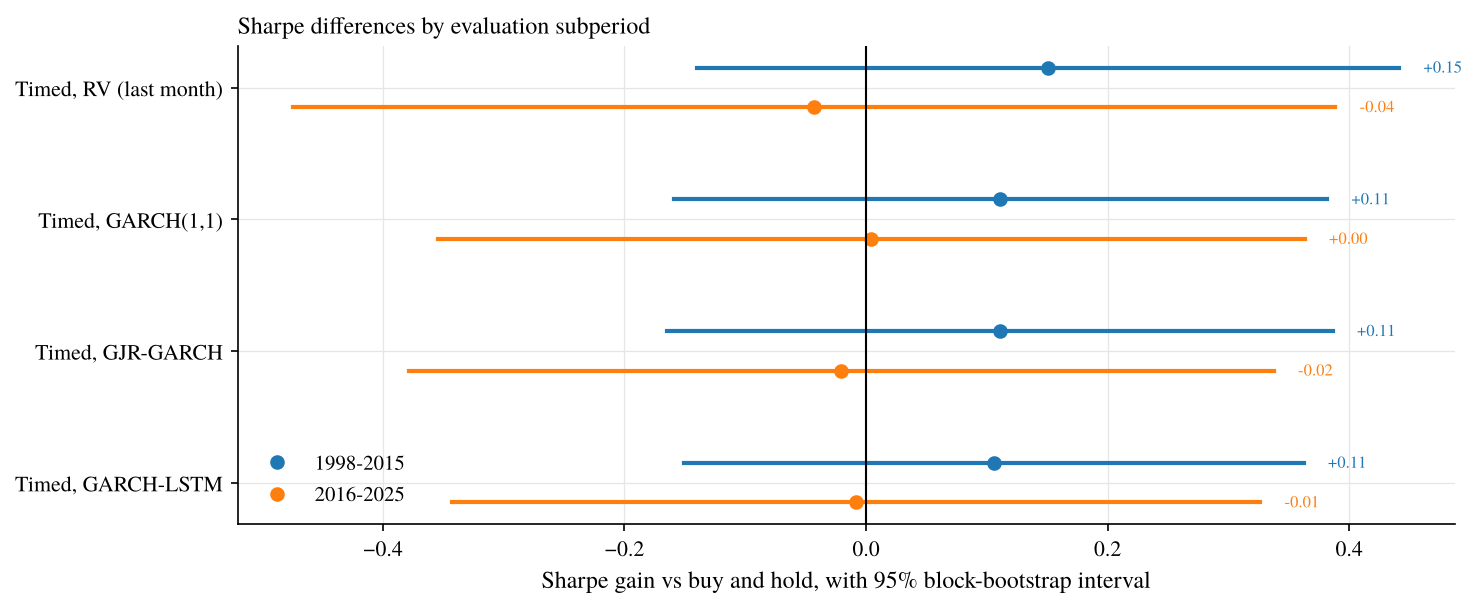
\includegraphics[width=0.75\textwidth]{figs/fig03_sharpe_by_period.png}
\caption{Sharpe gain over buy and hold with 95\% block-bootstrap intervals, 1998--2015 against 2016--2025.}
\label{fig:byperiod}
\end{figure}

\FloatBarrier
\subsection{Q2: does a better forecast give a better portfolio?}\label{sec:q2}
We keep the rule, the cap, the January reset of $c$ and the 10 bp costs fixed and order the forecasts from least to most accurate (Table~\ref{tab:ablation}, Figure~\ref{fig:mtvt}). The forecasts come from two estimation procedures (Section~\ref{sec:design}), so this compares forecasting procedures rather than isolating accuracy alone; the calibration check in Section~2.4 shows that the way $c$ is set does not affect the result.

VT is above 1 for every forecast (1.21 to 1.29): the risk side works whatever the forecast. MT, however, falls as accuracy rises: 1.006 for RV, 0.974 for GARCH(1,1), 0.95 for GJR-GARCH and the GARCH-LSTM, and 0.896 for \VIX. The extremes make the point: RV, the least accurate forecast, has the highest Sharpe ratio; \VIX, the most accurate, has the lowest. Among the three models the differences are small (Sharpe 0.597 to 0.608), and the GARCH-LSTM, despite its network, is only slightly more accurate than its GJR base and gives the same Sharpe ratio. \VIX{} is worst on both sides; its variance risk premium predicts returns positively (Bollerslev et al., 2009). The drawdown at equal volatility also deteriorates step by step as accuracy rises, from $-$32\% to $-$46\%. Five forecasts show an association, not proof that accuracy causes it. \textit{Answer to Q2: no.}

\begin{table}[htbp]
\centering\small
\caption{The forecasts ordered from least to most accurate, 1998--2025. MT and VT from eq.~\eqref{eq:mtvt}, before costs.}\label{tab:ablation}
\begin{adjustbox}{max width=\linewidth}\begin{tabular}{@{}lcccccc@{}}
\toprule
Forecast (least to most accurate) & QLIKE & Sharpe (net) & Sortino (net) & MT & VT & Max DD, equal vol, \%\\
\midrule
Buy and hold & -- & 0.516 & 0.748 & 1.000 & 1.000 & $-$50.3\\
RV (Moreira--Muir rule) & 0.454 & 0.612 & 0.919 & 1.006 & 1.245 & $-$32.0\\
GARCH(1,1) & 0.297 & 0.608 & 0.909 & 0.974 & 1.269 & $-$36.9\\
GJR-GARCH & 0.284 & 0.597 & 0.891 & 0.948 & 1.285 & $-$39.8\\
GARCH-LSTM & 0.280 & 0.597 & 0.889 & 0.949 & 1.285 & $-$41.8\\
\VIX{} (control) & 0.275 & 0.545 & 0.791 & 0.896 & 1.207 & $-$46.3\\
\bottomrule
\end{tabular}\end{adjustbox}
\end{table}

\begin{figure}[htbp]
\centering
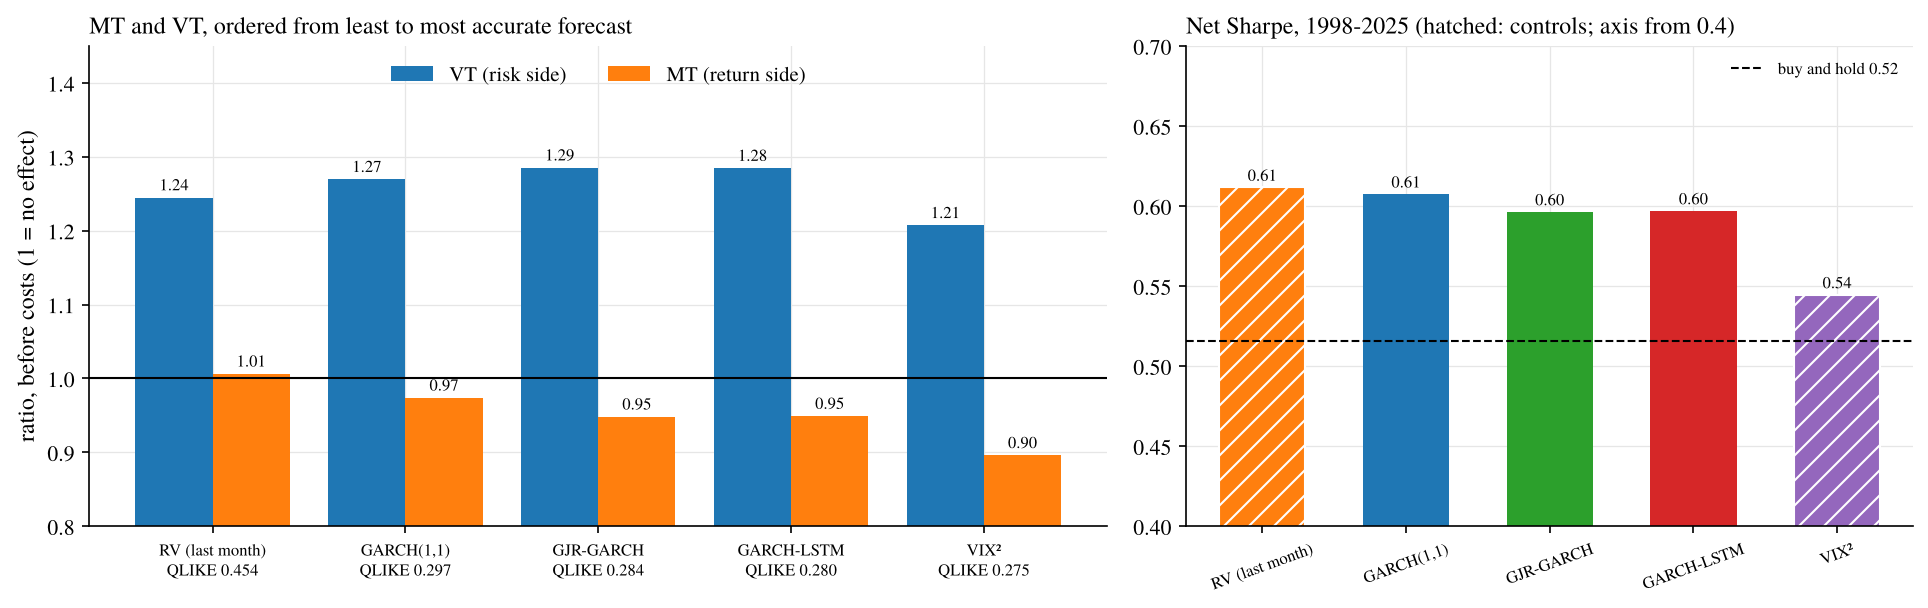
\includegraphics[width=0.95\textwidth]{figs/fig04_mt_vt.png}
\caption{Left: mean timing (MT) and variance timing (VT), from least to most accurate forecast. Right: net Sharpe ratio (hatched: controls).}
\label{fig:mtvt}
\end{figure}

\FloatBarrier
\subsection{Why not? Variance is predictable, returns are not}\label{sec:why}
\paragraph{What can be forecast?} We give returns and variance the same real-time test: an expanding-window predictive regression, re-estimated every month on all available data from 1970, forecasting next month over 1998--2025, with the out-of-sample $R^2$ measured against the historical average (Campbell and Thompson, 2008; Welch and Goyal, 2008) and the one-sided Clark and West (2007) test (Table~\ref{tab:oos}, Figure~\ref{fig:predict}).

\begin{table}[htbp]
\centering\small
\caption{Out-of-sample $R^2$ against the historical average, next month, 1998--2025. The GJR-GARCH and GARCH-LSTM regressions start in 1975, when their forecasts begin.}\label{tab:oos}
\begin{adjustbox}{max width=\linewidth}\begin{tabular}{@{}llcc@{}}
\toprule
Real-time predictor & Target & OOS $R^2$, \% & Clark--West $p$\\
\midrule
GARCH(1,1) forecast & log realised variance & 53.1 & 0.000\\
GJR-GARCH forecast & log realised variance & 53.6 & 0.000\\
GARCH-LSTM forecast & log realised variance & 53.6 & 0.000\\
RV (last month) & log realised variance & 47.1 & 0.000\\
\VIX & log realised variance & 57.1 & 0.000\\
Last month's return & excess return & $-$0.3 & 0.43\\
Past 12 months' return (Moskowitz et al., 2012) & excess return & $-$0.3 & 0.63\\
GARCH(1,1) variance forecast & excess return & $-$2.1 & 0.60\\
Average of the three (Rapach et al., 2010) & excess return & $-$0.6 & 0.57\\
Average, forecast $\ge 0$ (Campbell and Thompson, 2008) & excess return & $-$0.2 & 0.57\\
\bottomrule
\end{tabular}\end{adjustbox}
\end{table}

\begin{figure}[htbp]
\centering
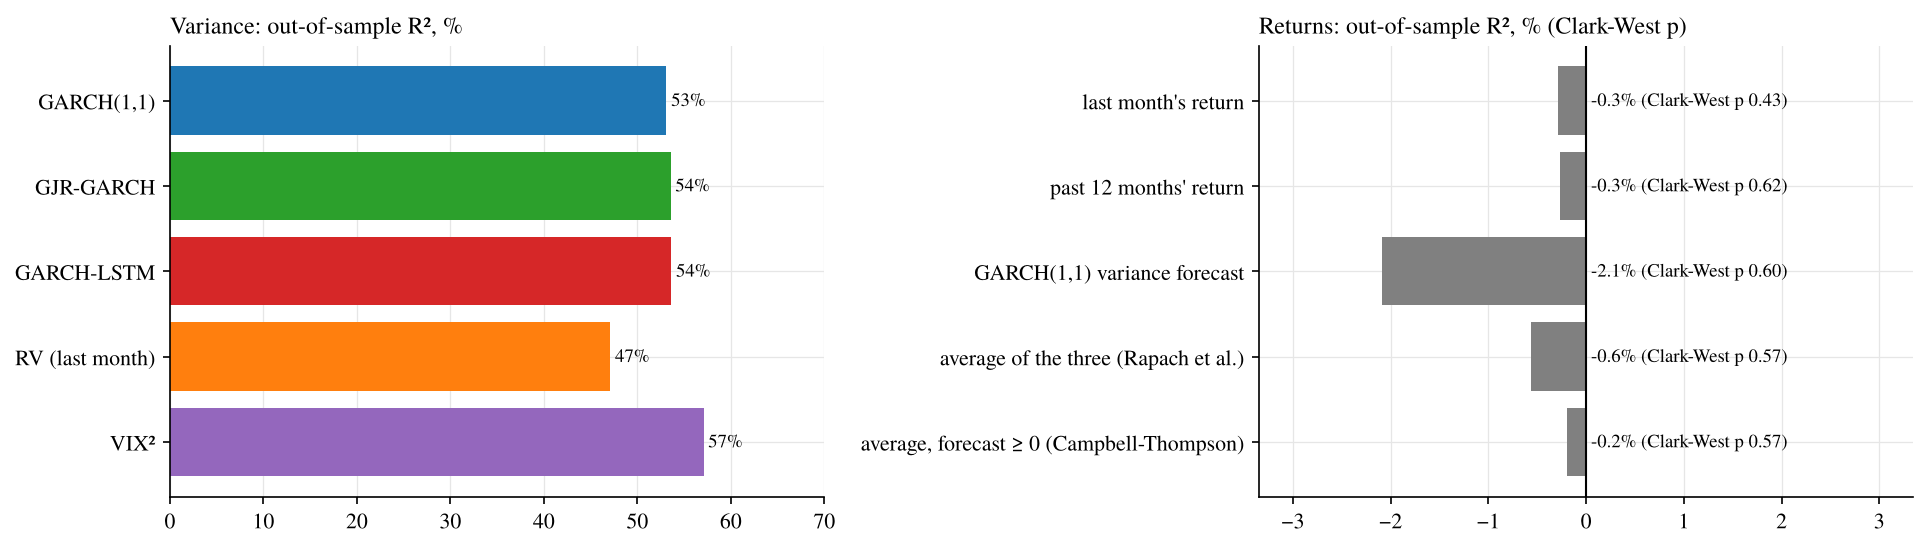
\includegraphics[width=0.95\textwidth]{figs/fig05_predictability.png}
\caption{What can be forecast one month ahead: variance (left) and returns (right); note the different scales.}
\label{fig:predict}
\end{figure}

The variance forecasts explain 47\% to 57\% of next month's log realised variance out of sample; for returns, every predictor does worse than the historical average equity premium. This is why the rule times only variance and treats the expected return as constant, and why a better variance forecast cannot raise MT: the rule has no information to tell the months that pay well from those that do not.

\paragraph{Where the return side leaks: the recovery months.} We split months in real time by last month's volatility: normal (not in its top 20\%, expanding window), panic (top 20\% and still rising, 5-day above 63-day variance) and recovery (top 20\% but already falling), for the Moreira--Muir rule over 1975--2025.

Recovery months have the highest average return (1.6\% a month), but the rule holds the same low exposure in panics and recoveries (0.34 and 0.35): an inverse-variance rule only sees the level of variance, which is high in both states (Table~\ref{tab:states}). A sharper variance forecast, which cuts exposure faster after a spike, makes this worse. The intervals are wide, so this is suggestive, and a simple fix (at least full exposure in recovery months) does not beat plain timing (Sharpe 0.59 against 0.61).

\begin{table}[htbp]
\centering\small
\caption{Market return and timed exposure by volatility state, 1975--2025 (timed on RV).}\label{tab:states}
\begin{adjustbox}{max width=\linewidth}\begin{tabular}{@{}lcccc@{}}
\toprule
State & Months & Market return, \%/month & Naive 95\% interval & Average exposure\\
\midrule
Normal & 434 & 0.64 & $\pm$0.36 & 1.20\\
Panic & 81 & 0.37 & $\pm$1.26 & 0.34\\
Recovery & 97 & 1.59 & $\pm$1.16 & 0.35\\
\bottomrule
\end{tabular}\end{adjustbox}
\end{table}

\FloatBarrier
\subsection{Q3: does training the forecast for the decision help?}\label{sec:q3}

\begin{table}[htbp]
\centering\footnotesize
\caption{Accuracy-trained (Acc) vs decision-trained (Dec) forecasts on six factors, 1998--2025. Every forecast goes through the full rule (cap 1.5, 10 bp, $c$ reset every January); GARCH-LSTM: ensemble of 5 seeds.}\label{tab:q3}
\setlength{\tabcolsep}{3.5pt}
\begin{adjustbox}{max width=\linewidth}\begin{tabular}{@{}lccccccccccccc@{}}
\toprule
 & B\&H & \multicolumn{4}{c}{Net Sharpe ratio} & \multicolumn{4}{c}{Realised objective, \% p.a.} & \multicolumn{4}{c}{QLIKE (diagnostic)}\\
\cmidrule(lr){3-6}\cmidrule(lr){7-10}\cmidrule(lr){11-14}
 & SR & \multicolumn{2}{c}{GJR} & \multicolumn{2}{c}{LSTM} & \multicolumn{2}{c}{GJR} & \multicolumn{2}{c}{LSTM} & \multicolumn{2}{c}{GJR} & \multicolumn{2}{c}{LSTM}\\
Factor & & Acc & Dec & Acc & Dec & Acc & Dec & Acc & Dec & Acc & Dec & Acc & Dec\\
\midrule
Mkt & 0.516 & 0.597 & 0.573 & 0.597 & 0.537 & 3.46 & 3.21 & 3.47 & 2.68 & 0.284 & 0.285 & 0.280 & 0.587\\
SMB & 0.111 & 0.002 & $-$0.063 & 0.006 & $-$0.079 & $-$1.48 & $-$2.04 & $-$1.45 & $-$2.99 & 0.192 & 0.198 & 0.188 & 0.322\\
HML & 0.080 & 0.052 & 0.057 & 0.051 & $-$0.068 & $-$0.93 & $-$0.96 & $-$0.95 & $-$2.07 & 0.338 & 0.445 & 0.339 & 0.449\\
Mom & 0.210 & 0.553 & 0.537 & 0.548 & 0.532 & 2.98 & 2.81 & 2.93 & 2.78 & 0.271 & 0.259 & 0.250 & 0.424\\
RMW & 0.367 & 0.321 & 0.321 & 0.319 & \textbf{0.427} & 1.02 & 1.02 & 1.01 & \textbf{1.79} & 0.193 & 0.226 & 0.194 & 0.709\\
CMA & 0.241 & 0.052 & 0.114 & 0.054 & 0.085 & $-$0.55 & $-$0.36 & $-$0.55 & $-$0.43 & 0.184 & 0.270 & 0.187 & 1.087\\
\bottomrule
\end{tabular}\end{adjustbox}
\end{table}

\begin{itemize}
\item \textbf{On its own objective, Dec loses.} This is the primary yardstick, since it is what Dec was trained to maximise. The decision-trained GARCH-LSTM beats the accuracy-trained network out of sample on only 2 of 6 factors (RMW $+$0.78, CMA $+$0.12\% a year) and is worse on average ($-$0.45\% a year). No difference is significant (bootstrap $p$ 0.12 to 0.81, unadjusted).
\item \textbf{On the Sharpe ratio it also loses.} Dec minus Acc is $-$0.06 on the market, $-$0.09 on SMB, $-$0.12 on HML and $-$0.02 on momentum, against $+$0.11 on RMW and $+$0.03 on CMA (average $-$0.02). After the Romano--Wolf adjustment over the 12 Sharpe comparisons no $p$-value for the GARCH-LSTM is below 0.70.
\item \textbf{The control.} For GJR-GARCH, with few parameters, Dec minus Acc in the Sharpe ratio is between $-$0.06 and $+$0.06 (average $-$0.01), and the realised objective is lower on 5 of 6 factors. Dec is slightly but consistently worse on the market ($-$0.023, bootstrap $p=0.017$) and SMB ($-$0.064, $p=0.025$); neither survives the Romano--Wolf adjustment ($p=0.13$ and $0.11$).
\item \textbf{On the market,} the decision-trained GARCH-LSTM is the weakest timed portfolio (Table~\ref{tab:perf}: Sharpe 0.537, volatility 12.8\%, worst drawdown $-$37.9\%). Its Sharpe gain over buy and hold is $+$0.02 ($p=0.84$; Ledoit--Wolf $p=0.84$), and against the accuracy-trained network $-$0.06 ($p=0.30$).
\item \textbf{The price: worse forecasts.} The decision-trained network's forecasts are 1.3 (HML) to 5.8 (CMA) times worse in QLIKE, and still 1.5 to 4.1 times worse after rescaling each forecast by its best constant, so Dec gives up tracking of volatility, not only calibration.
\item \textbf{The network adds little even when trained for accuracy.} The accuracy-trained GARCH-LSTM and GJR-GARCH have almost the same Sharpe ratio on every factor (within 0.005).
\end{itemize}
\textit{Answer to Q3: no.} Decision-focused learning accepts a worse forecast in exchange for a better decision; here the network pays the price without obtaining the benefit. This tests one design, not decision-focused learning in general.

\begin{figure}[htbp]
\centering
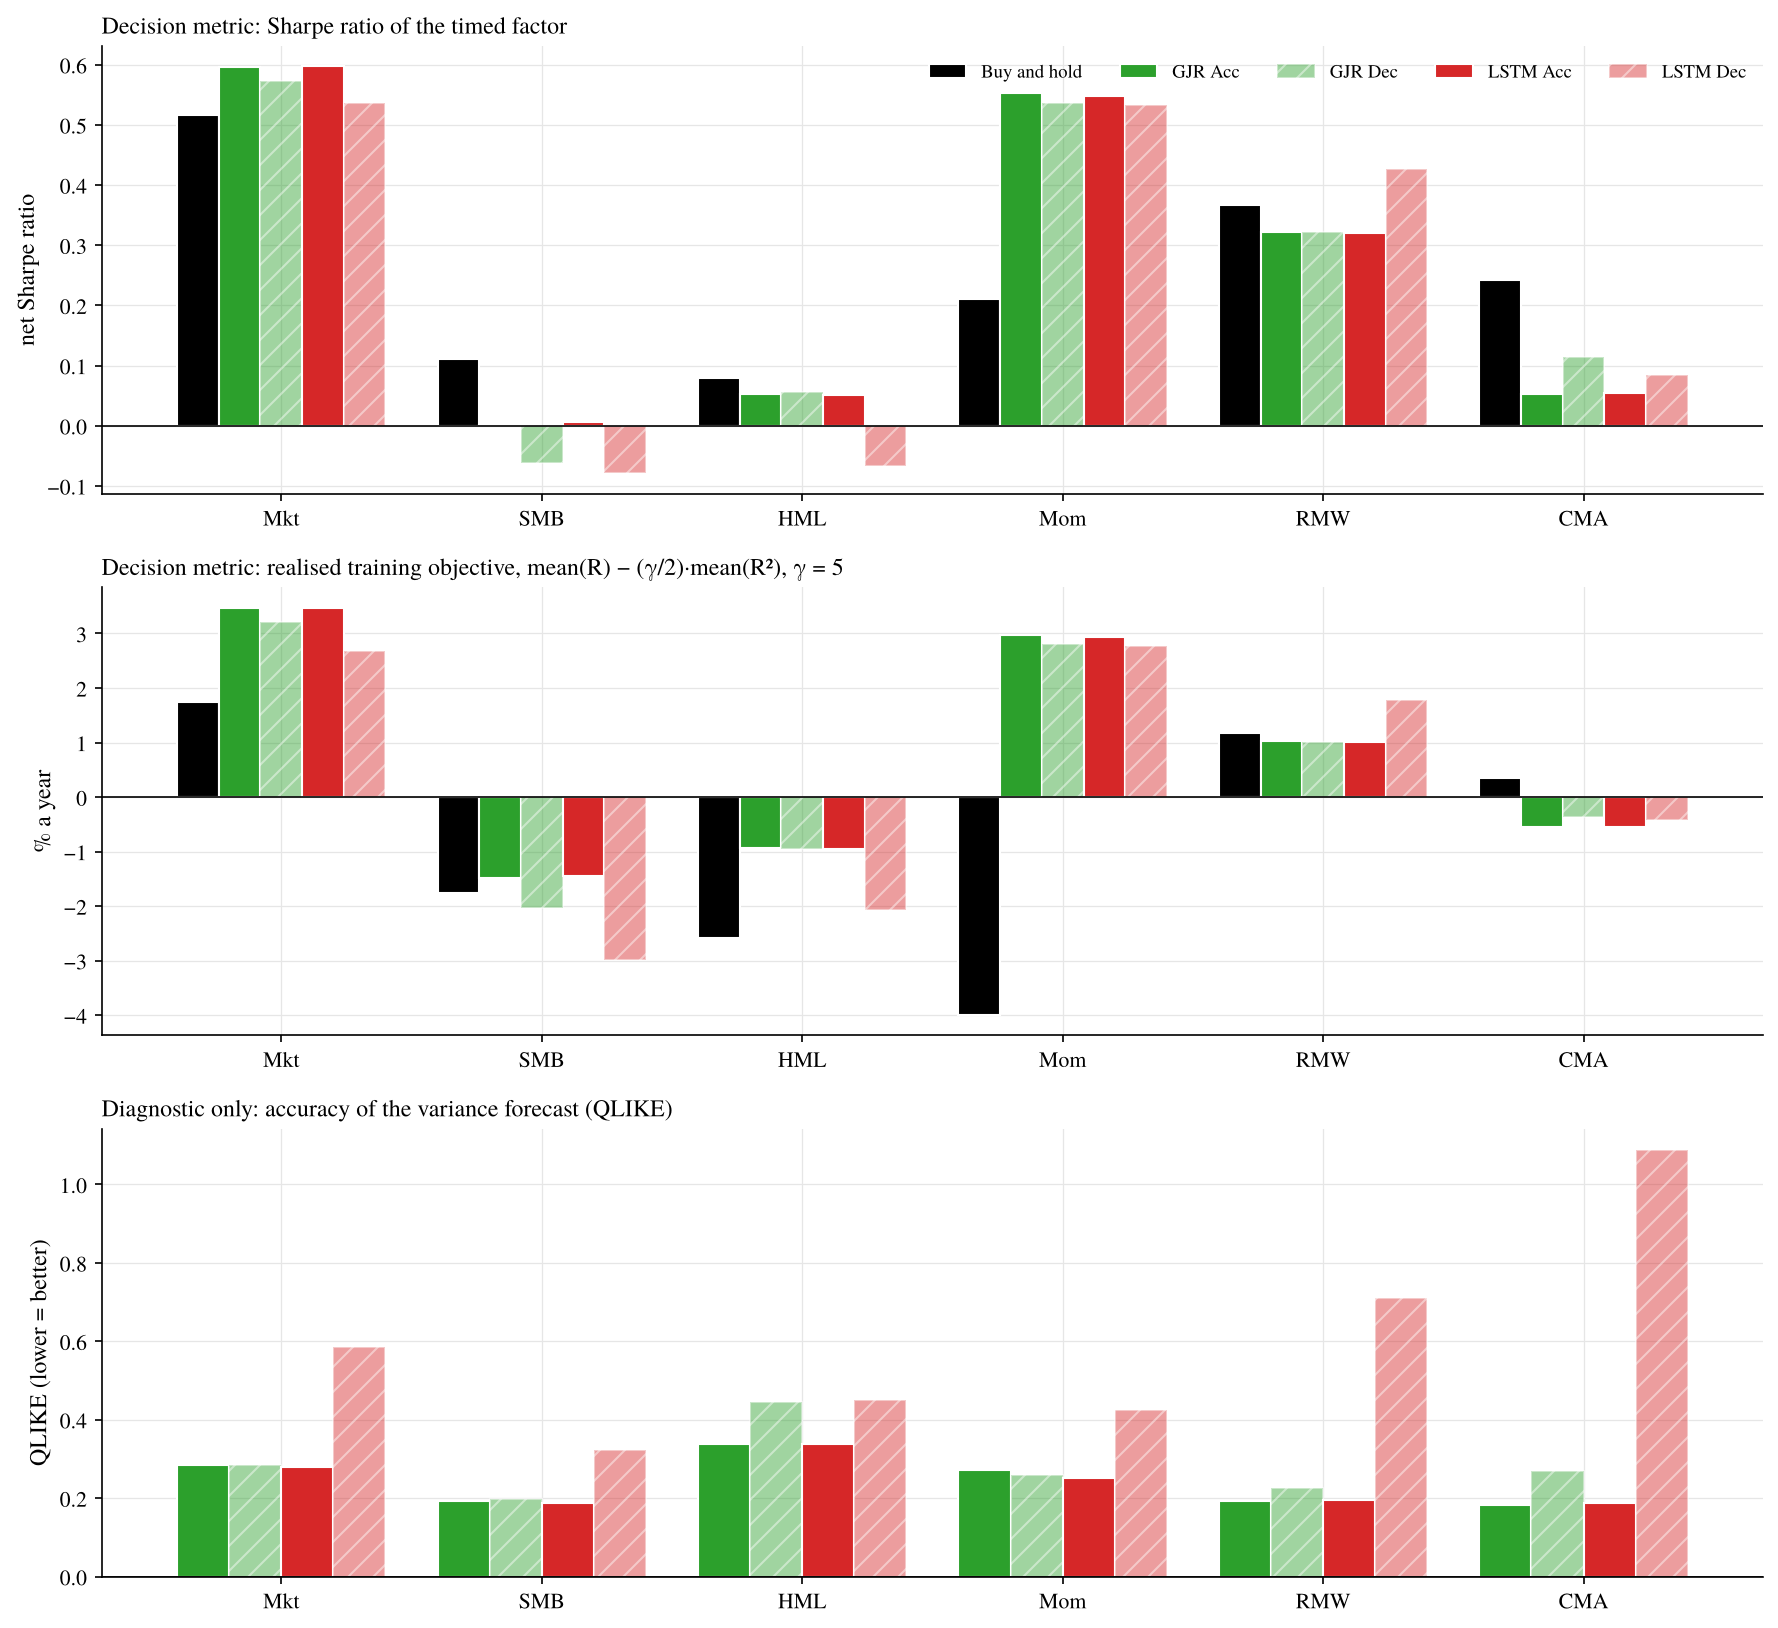
\includegraphics[width=0.9\textwidth]{figs/fig06_acc_vs_dec.png}
\caption{Acc vs Dec: net Sharpe ratio, realised training objective and QLIKE on the six factors, 1998--2025.}
\label{fig:accdec}
\end{figure}

\FloatBarrier
\subsection{Other benchmarks}\label{sec:otherbench}

\begin{table}[htbp]
\centering\small
\caption{Common window of the course CRSP file, February 2000 -- December 2020. Timed portfolios net of costs; passive benchmarks without costs. ``At market vol'': each series rescaled after the fact to the market's volatility.}\label{tab:bench}
\begin{adjustbox}{max width=\linewidth}\begin{tabular}{@{}lcccccc@{}}
\toprule
Portfolio & Sharpe & Sortino & Vol, \% & Max DD, \% & Max DD at market vol, \% & Vol of vol, \%\\
\midrule
Buy and hold (S\&P 500 proxy) & 0.435 & 0.624 & 15.8 & $-$50.3 & $-$50.3 & 6.1\\
EW six factors & \textbf{0.752} & \textbf{1.206} & 4.6 & $-$12.2 & $-$37.4 & 2.1\\
EW CRSP stocks & 0.497 & 0.770 & 22.1 & $-$59.0 & $-$45.7 & 8.8\\
Timed, RV & 0.558 & 0.821 & 10.7 & $-$21.3 & $-$32.6 & 3.1\\
Timed, GARCH(1,1) & 0.560 & 0.825 & 10.8 & $-$25.1 & $-$37.2 & 2.9\\
Timed, GJR-GARCH & 0.562 & 0.829 & 10.8 & $-$26.3 & $-$38.6 & 2.7\\
Timed, GARCH-LSTM & 0.560 & 0.822 & 11.2 & $-$28.7 & $-$40.4 & 2.6\\
\bottomrule
\end{tabular}\end{adjustbox}
\end{table}

Over 2000--2020 the equal-weighted factor mix has by far the best Sharpe ratio (0.75), ahead of the timed market portfolios (0.56), the equal-weighted CRSP stocks (0.50) and the market (0.44). At the market's volatility the timed portfolios lose 33\% to 40\% at worst against 50\% for the market, 46\% for the CRSP stocks and 37\% for the factor mix. Timing beats the market on risk, but diversifying across factors does more for the Sharpe ratio.
